Các mẫu chiến lược phân tích nghiệp vụ kinh doanh đưa ra việc phân chia các thành phần và hiểu mối quan hệ của các thành phần đó.


Đưa ra phân tách thành các 
%
 
Tuy nhiên, giai đoạn thiết kế chiến lược rất quan trọng trong việc thiết lập sự hiểu biết chung về miền giữa chuyên gia miền và nhóm phát triển, 

được thiết kế để giúp các nhà phát triển giải quyết những thách thức thiết kế cụ thể thường gặp trong các miền phức tạp
xác định các quy tắc kinh doanh quan trọng, 

Việc thiết kế chiến lược giúp định hình sự hiểu biết chung và xác định các quyết định quan trọng về kiến ​​trúc.
, và đảm bảo rằng kiến trúc phần mềm phản ánh đúng các yêu cầu kinh doanh.


%

Mục tiêu của thiết kế chiến lược là tạo ra một kiến trúc phần mềm gắn kết và có thể 
% mở rộng,
 phù hợp với các mục tiêu kinh doanh và cung cấp nền tảng vững chắc cho sự phát triển và tăng trưởng trong tương lai.

%

Các mẫu chiến lược đề cập đến thiết kế tổng thể của hệ thống bao gồm:

\begin{itemize}

\item Muc1

\item Muc2

\item các mục bên dưới \dots

\end{itemize}

%

\begin{figure}[H]

\centering

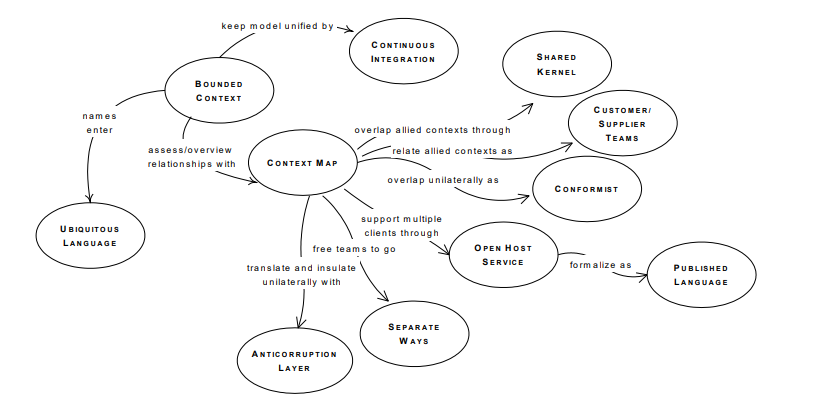
\includegraphics[width = 1\textwidth]{pictures/CacMoHinhChienLuoc/temp.png}

\caption{Sơ đồ   về các thành phần trong mô hình chiến lược}

\end{figure}

%!<! - - $ Vẽ lại sau: - - >

%!<! - - $ Vẽ lại sau: - - >

%!<! - - $ Vẽ lại sau: - - >

%!<! - - $ Vẽ lại sau: - - >

%!<! - - $ Vẽ lại sau: - - >

%!<! - - $ Vẽ lại sau: - - >

%!<! - - $ Vẽ lại sau: - - >

%!<! - - $ Vẽ lại sau: - - >

%!<! - - $ Vẽ lại sau: - - >

%!<! - - $ Vẽ lại sau: - - >

%!<! - - $ Vẽ lại sau: - - >

%!<! - - Bối cảnh giới hạn (Bounded Context) - - >

%!<! - - [Giữ cho mô hình thống nhất] Tích hợp Liên tục (Continuous Integration) - - >

%!<! - - [Tính nhất quán trong trao đổi] Ngôn ngữ chung (Ubiquitous Language) - - >

%!<! - - [Tổng quan mối quan hệ] Bản đồ bối cảnh (Context Maps) - - >

%!<! - - Symmetric Relationship: Separate ways, Shared Kernel - - >

%!<! - - Asymmetric Relationship: Customer - Supplier, Conformist, Anti Corruption Layer - - >

%!<! - - - - >

%!<! - - One - to - Many Relationship: Open Host Service, Published Language - - >

%!<! - - dịch và cách ly đơn phương với - - >

%!<! - - [lớp] lớp (Context Maps) - - >

%

%!<! - - "Bản đồ bối cảnh dịch chuyển và cách ly một cách đơn phương để tạo thành cấu trúc lớp." - - >

%!<! - - Tách biệt - - >

